\documentclass{article}
\usepackage[utf8]{inputenc}
\usepackage{amsmath, amssymb, amsthm}
\usepackage{titlesec}
\usepackage{graphicx}
\usepackage[dvipsnames]{xcolor}
\usepackage{listings}
\usepackage{lastpage}
\usepackage{tabularx}
\usepackage{mathtools}
\usepackage[thinc]{esdiff}


% Customization -------

% Paper size, margin
\usepackage[letterpaper,top=1.5cm,bottom=1.5cm,left=1.75cm,right=1.75cm,heightrounded]{geometry}

% line height
\renewcommand{\baselinestretch}{1.15} % line space

% Paragraph indentation 
\setlength{\parindent}{0pt} % no indent

% Paragraph spacing
\setlength{\parskip}{0.8em} % space between paragraphs

% Equation numbering per section
\counterwithin*{equation}{section}
\counterwithin*{equation}{subsection}

% Graphics path
\graphicspath{ {./images/} }

% --------------------

\title{ECE355: Lecture 17}
\author{Farbod Mohammadzadeh\\
    (1008360462)\\}
\date{13 October 2023\\ \pageref{LastPage} Pages}

\begin{document}
\Large
\maketitle
{\normalsize \tableofcontents}
\newpage
\section{ch. 3.5: \underline{Properties of Continuous Time Fourier Series (CTFS)}}
Suppose we have the CTFS coefficients $\{a_k\}_{k= - \infty , \infty}$ of some signal, $x(t)$.

How can we find the CTFS coefficients of signals obtained by simple manipulations, e.g, $3x(t)+2$, $x(t-5)$, $Re\{x(t)\}$, $\diff{f}{x}$, $\dots$?

{\color{ForestGreen} There are many useful propertied of CTFS that you can use as shortcuts to find the CTFS coefficients for these transformed signals}

First, for convenience, let's use a shorthand notation to indicate the relationship between a periodic signal. \& its CTFS coefficients.
\begin{align}
    x(t)                      & \xleftrightarrow[]{\text{FS}} a_k \\
    x(t)                      & \ - \text{CT Periodic}            \\
    T                         & \ - Fundemental Period            \\
    \omega_0 = \frac{2\pi}{T} & \ - Fundemental Frequency
\end{align}

\subsection{Linearity:}
If $y(t)$ has a fundamental period T {\color{ForestGreen}(Same as $x(t)$)}:

Then:
\begin{equation}
    Ax(t) + By(t) \xleftrightarrow[]{FS}{Aa_k + Bb_k}
\end{equation}

\subsubsection{\underline{Proof:}}
\begin{align}
    \text{LHS} & = A (\sum^{\infty}_{k= - \infty} a_k e^{jk \omega_0 t}) + B (\sum^{\infty}_{k= - \infty} b_k e^{jk \omega_0 t}) \\
               & =\sum^{\infty}_{k= - \infty} (Aa_k + Bb_k) e^{jk \omega_0 t}
\end{align}


\subsection[]{Time Shifting:}

\begin{equation}
    x(t-t_0) \xleftrightarrow[]{FS}{a_k e^{-jk \omega_0 t_0}}
\end{equation}
Here there is no change to the magnitude of the FS coefficients.

\subsubsection{\underline{Proof:}}
Finding FS coefficients for $x(t-t_0)$:

\begin{align}
     & = \frac{1}{T} \int^{}_{T} x(t-t_0) e^{-jk \omega_0 t} dt                                               \\ \tau = t-t_0 \rightarrow
     & = \frac{1}{T} \int^{}_{T} x(\tau) e^{-jk \omega_0 (\tau + t_0)} d\tau                                  \\
     & = e^{-jk \omega_0 t_0} {\color{red}\underbrace{\frac{1}{T} \int^{}_{T} x(\tau) e^{-jk \omega_0 \tau} d\tau}_{ = a_k}} \\
     & = a_k e^{-jk \omega_0 t_0}
\end{align}

\subsubsection[]{\underline{Example:}}
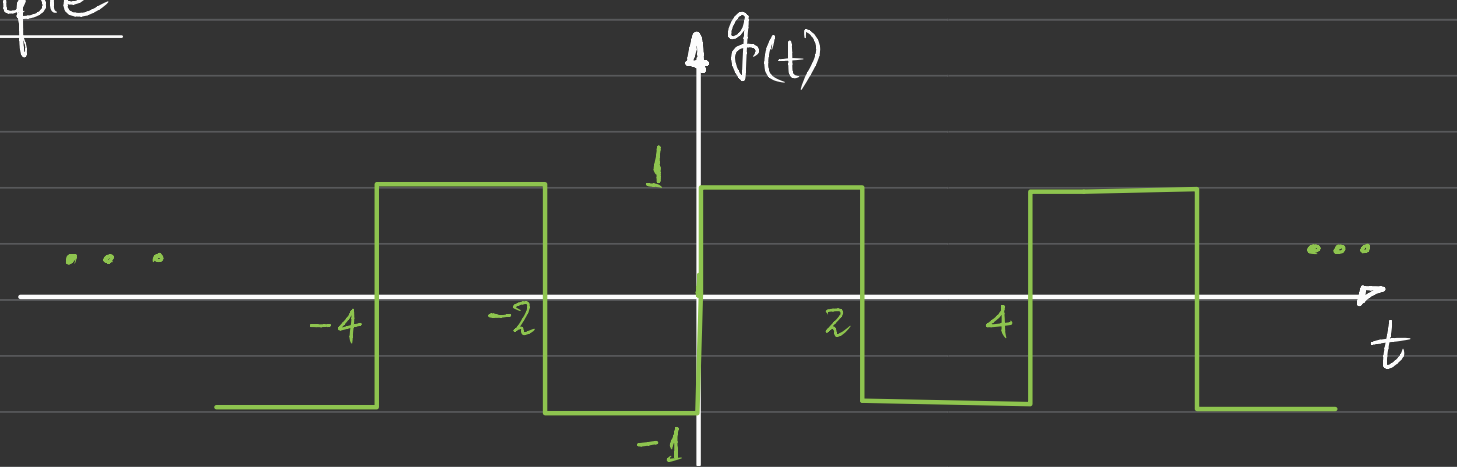
\includegraphics[width=\textwidth]{1.2.2example}
- To evaluate its FS coefficients. recall the examsple of lecture 15.

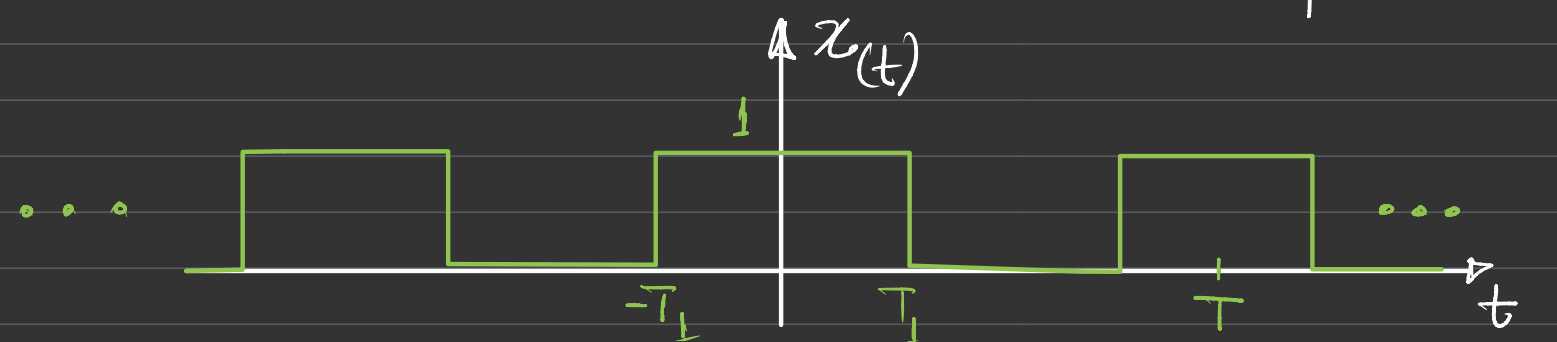
\includegraphics[width=\textwidth]{1.2.2example2}

{\huge \begin{equation}
        FS \xrightarrow{} a_k =  \left\{
        \begin{array}{ll}
            \frac{\sin(\frac{k\pi}{2})}{k\pi} & , \ k \neq 0 \\
            \frac{x-a}{b-a}                   & , \ k = 0
        \end{array}
        \right.
    \end{equation}}
- Relating $g(t)$ to $x(t)$: Let $T = 4$ and $\omega_0 = \frac{2\pi}{4} = \frac{\pi}{2}$. \&
\begin{equation}
    g(t) = \underbrace{2x (t-1)}_{\mathbf{I}} \underbrace{-1}_{\mathbf{II}} \leftrightarrow C_k
\end{equation}

{\color{red}\begin{align}
    \mathbf{I.} \   & 2x (t-1)  \xleftrightarrow[]{FS} 2a_k e^{-jk\frac{\pi}{2}} \\
    \mathbf{II.} \  & -1 x \xleftrightarrow[]{FS}
    \left\{\begin{array}{ll}
               -1 & , \ k \neq 0 \\
               0  & , \ k = 0
           \end{array}
    \right |\text{using FS analysis equation}
\end{align}}

\begin{equation}
    \therefore \ \mathbf{I \ \& \ II} \xrightarrow{}
    \left\{\begin{array}{ll}
        c_0 = 2a_0 -1 = 1-1 =0                                           & ; \ k=0     \\
        c_k = 2 e^{-jk \frac{\pi}{2}} \frac{\sin(k\frac{k\pi}{2})}{k\pi} & ; \ k\neq 0
    \end{array}\right.
\end{equation}

\subsection{Time Scaling:}
For $\alpha > 0 $ , $x(\alpha t) \xleftrightarrow[]{FS} a_k$ , with fundamental frequency, $\alpha \omega_0$

\subsubsection{\underline{Proof:}}

\begin{align}
    x(\alpha t) & =\sum^{\infty}_{k= - \infty} a_k e^{jk\omega_0 (\alpha t)}                                                                   \\
                & =\sum^{\infty}_{k= - \infty} a_k e^{jk\underbrace{(\alpha \omega_0)}_{\text{Fundemental frequency is now }\alpha \omega_0}t}
\end{align}

\subsection{Time Reversal: }

\end{document}